\documentclass[12pt]{article}

%% \usepackage{fancyhdr}: This package is used for customizing the page headers and footers in a document.

%% \usepackage{parskip}: This package is used to alter the spacing between paragraphs. It usually sets zero indentation and adds some space between paragraphs for better readability.

%% \usepackage{changepage}: This package provides environments for changing the layout of single pages. It can be used for making temporary adjustments to page margins or other layout settings.

%% \let\cleardoublepage=\clearpage: This line redefines the \cleardoublepage command to have the same behavior as the standard \clearpage command. \cleardoublepage normally ends the current page and starts a new one, ensuring that the next page begins on a right-hand (odd-numbered) page in double-sided documents.

%% \usepackage{ragged2e}: This package is an enhanced version of the standard \raggedright and \raggedleft commands. It provides more advanced options for controlling text alignment.

%% \usepackage{makecell}: This package provides the \makecell command. This command allows for line breaks within cells of tables and provides other enhancements for formatting cells in tables.

%% \makeatletter: This command changes the category code of the at symbol (@) to 11, allowing it to be used in command names. In LaTeX, commands with @ in their names are typically meant for internal use and should not be accessed or modified by users directly. However, within a \makeatletter and \makeatother pair, you can use @ in command names.

%% \setlength{\@fptop}{0pt}:  This line sets the length parameter \@fptop to 0pt. The \@fptop length controls the space above a float placed at the top of a page. By setting it to 0pt, you are essentially minimizing the vertical space between the top of the page and the top of the float.

%% \makeatother: This command changes the category code of the at symbol back to 12, restoring its usual behavior. This is done to prevent accidental or unintended use of @ in command names outside of the intended scope.

%% \usepackage[subpreambles=true]{standalone}: This package provides the \input and \include commands with additional options for including standalone documents. When used with the subpreambles=true option, it allows the preambles (i.e., document settings and packages) of the standalone files to be processed individually. This is useful when you have multiple standalone documents that are later included in a main document.

%% \usepackage{import}: The import package enhances the \import command, allowing you to import files from different directories and manage file paths more conveniently. It is often used in conjunction with the standalone package to include standalone documents located in different directories.

%% \usepackage{subfiles}: This package facilitates the creation of modular LaTeX documents. It allows you to compile both the main document and individual subfiles independently. When a subfile is included in the main document, it is treated as if it were a standalone document. This makes it easier to work on different parts of a document separately, and it helps avoid recompiling the entire document every time a small change is made.

%% \usepackage{smartdiagram}: The smartdiagram package in LaTeX is designed to create various types of diagrams, charts, and flowcharts with a simple and flexible syntax. It provides an easy way to generate visually appealing and informative diagrams without having to manually draw them. The package is particularly useful for creating flowcharts, concept maps, and other types of diagrams commonly used in educational materials, presentations, and documents.

%% \usepackage[bottom]{footmisc}: This line includes the footmisc package with the option [bottom]. The footmisc package provides customization options for footnotes in LaTeX documents. The [bottom] option ensures that footnotes are placed at the bottom of the page, rather than being positioned in the default location (usually at the bottom of the text area).

%% \setlength\footnotemargin{10pt}: This line sets the length parameter \footnotemargin to a value of 10pt. The \footnotemargin controls the indentation of the first line of footnotes. By setting it to 10pt, you are specifying a horizontal space of 10 points (1/72.27 inch) for the indentation of the first line of each footnote.

%% \usepackage{pifont}: The \usepackage{pifont} line in LaTeX is used to include the pifont package. The pifont package provides access to a variety of symbols and dingbat characters (ornaments) that are not part of the standard set of LaTeX symbols. One of the notable features of the pifont package is the availability of commands for accessing special symbols represented by numbers. For example, you can use \ding{1}, \ding{2}, and so on, to insert different types of symbols or characters.

%%%%%%%%% Graphics-related packages %%%%%%%%%

%% \usepackage{graphicx}: This package allows you to include graphics (images) in your document.

%% \usepackage{float}: The float package improves the placement of figures and tables.

%% \usepackage{caption}: The caption package enhances the customization of captions for figures and tables.

%% \usepackage{pdfpages}: This package enables the inclusion of entire PDF pages into your document. 

%% \usepackage{pdflscape}: The pdflscape package provides support for landscape pages in PDF output.

%%%%%%%%% Document formatting and layout packages %%%%%%%%%

%% \usepackage{array}: This package extends the functionality of the array and tabular environments for better control over column formatting in tables.

%% \usepackage{indentfirst}: The indentfirst package indents the first paragraph after a section heading.

%% \usepackage{amsmath}: This package provides enhanced support for mathematical typesetting.

%% \usepackage{url}: The url package allows for the typesetting of URLs with proper line breaking.

%% \usepackage{verbatim}: The verbatim package provides the verbatim environment for displaying text exactly as entered, without any formatting.

%%%%%%%%% Table of contents and bibliography packages %%%%%%%%%

%% \usepackage{bookmark}: This package enhances the functionality of bookmarks in a PDF document.

%% \usepackage[numbib,nottoc]{tocbibind}: The tocbibind package is used to include the bibliography in the table of contents and control the depth of inclusion for other sections.

%%%%%%%%% Table of contents formatting %%%%%%%%%

%% \usepackage{tocloft}: The tocloft package provides additional customization options for the table of contents.

%%%%%%%%% Page numbering and references %%%%%%%%%

%% \usepackage[lastpage, user]{zref}: The zref package is used for referencing page numbers. The lastpage option allows you to refer to the last page number, and the user option enables the user to define custom properties.


%%\usepackage[letterpaper,                 Specifies that the paper size should be letter.
%%            bindingoffset=0.2in,            It is the space added to the left margin for binding purposes.
%%            left=1in,                            Sets the left margin of the page to 1 inch.
%%            right=1in,                          Sets the right margin of the page to 1 inch.
%%            top=1in,                            Sets the top margin of the page to 1 inch.
%%            bottom=1in,                      Sets the bottom margin of the page to 1 inch
%%            footskip=.25in]{geometry}  Specifies the distance from the bottom of the text block 
%%                                                    to the baseline of the footer. It sets the space between the text 
%%                                                    and the footer.


%%\renewcommand{\cftsecfont}{\bfseries} % Font style

%%\renewcommand{\cftsecleader}{\cftdotfill{\cftdotsep}} %% Dotted lines for sections

%%\renewcommand{\cftsubsecleader}{\cftdotfill{\cftdotsep}} %% Dotted lines for subsections

%%\renewcommand{\cftsecafterpnum}{\hfill} % Align page number to the right

% Add a horizontal rule after the TOC title
%%\renewcommand{\cftaftertoctitle}{\par\noindent\hrulefill\par}

% Customize the appearance of table entries in the LOT
%%\renewcommand{\cfttabfont}{\bfseries} % Font style for tables
%%\renewcommand{\cfttableader}{\cftdotfill{\cftdotsep}} % Dots between entry and page number for %tables
%%\renewcommand{\cfttabafterpnum}{\hfill} % Align page number to the right for tables
%%\renewcommand{\cftafterlottitle}{\par\noindent\hrulefill\par} % Add a horizontal rule after the LOT title

% Customize the appearance of figure entries in the LOF
%%\renewcommand{\cftfigfont}{\bfseries} % Font style for figures
%%\renewcommand{\cftfigleader}{\cftdotfill{\cftdotsep}} % Dots between entry and page number for %figures
%%\renewcommand{\cftfigafterpnum}{\hfill} % Align page number to the right for figures
%%\renewcommand{\cftafterloftitle}{\par\noindent\hrulefill\par} % Add a horizontal rule after the LOF title

%%---------------------Beginning of Research Paper Preamble-----------------------%%

\usepackage[toc,page]{appendix}
\usepackage{multicol}
\usepackage{multirow}
\usepackage{subcaption}
\usepackage[table,dvipsnames]{xcolor}
\usepackage{parskip}
\usepackage{changepage} % Allows for the adjustment of text height, text width, margins, column %%%separation, headers, and footers
\let\cleardoublepage=\clearpage
\usepackage{ragged2e}  % Allows different justification schemes for various cells of the table
%%\usepackage{makecell}

\makeatletter
\setlength{\@fptop}{0pt}
\makeatother


%%-------Define colors for Cost Boxes-----------------------------%%
\usepackage[table]{xcolor}
\usepackage{colortbl}
\definecolor{white}{RGB}{255, 255, 255}

%%---------------------------------------------------------------------%%



%%---------Compile documents from multiple files---------------%%
%\usepackage[subpreambles=true]{standalone}
\usepackage{import}
\usepackage{subfiles}
%%-----------------------------------------------------------------------%%

%%----------------------------Diagramming---------------------------%%
\usepackage{smartdiagram}
%%-----------------------------------------------------------------------%%

%%--------------------For adjustwidth environment----------------%%
\usepackage{changepage}
%%-----------------------------------------------------------------------%%

%%-----------------------Footnotes------------------------------------%%

\usepackage[bottom,hang]{footmisc}
\setlength\footnotemargin{10pt}
\renewcommand\thefootnote{\textcolor{orange}{\arabic{footnote}}}
%%----------------------------------------------------------------------%%

%%---------------Margin notes---------------------------------------%%

%\usepackage{todonotes}
%\newcommand{\todoredefined}[2][]
%{\todo[noline,color=red, #1]{#2}}
 
%%----------------Fonts------------------------------------------------%%
\usepackage{pifont} % More styles for bullets


%%---------------Graphics, page geometry, headers, pdf, tocbibind----------%%
\usepackage{graphicx, array, indentfirst, float, caption, pdfpages, pdflscape, amsmath,
url, verbatim, fancyhdr, fancybox, lipsum}

\usepackage{bookmark}
\usepackage{booktabs}

\usepackage[numbib,nottoc]{tocbibind}

\usepackage{tocloft}

\usepackage[
lastpage, user]{zref} % For hyperref feature

\usepackage[usegeometry]{typearea}% load before geometry

\usepackage[letterpaper,
            bindingoffset=0.2in,
            left=1in,
            right=1in,
            top=1in,
            bottom=1in,
            footskip=.25in]{geometry}

\usepackage{fancyhdr} 
\pagestyle{fancy}{%
\fancyhf{}
\fancyhead[R]{\thepage}
}


%%\geometry{
%%a4paper,
%%total={170mm,257mm},
%%left=20mm,
%%top=20mm
%%}


%%----------Add dotted lines to the table of contents-----------------------%%

%\renewcommand{\cftsecfont}{\bfseries} % Font style

\renewcommand{\cftsecleader}{\cftdotfill{\cftdotsep}} %% Dotted lines for sections

\renewcommand{\cftsubsecleader}{\cftdotfill{\cftdotsep}} %% Dotted lines for subsections

%\renewcommand{\cftsecafterpnum}{\hfill} % Align page number to the right

% Add a horizontal rule after the TOC title
%\renewcommand{\cftaftertoctitle}{\par\noindent\hrulefill\par}

% Customize the appearance of table entries in the LOT
%\renewcommand{\cfttabfont}{\bfseries} % Font style for tables
\renewcommand{\cfttableader}{\cftdotfill{\cftdotsep}} % Dots between entry and page number for tables
%\renewcommand{\cfttabafterpnum}{\hfill} % Align page number to the right for tables
%\renewcommand{\cftafterlottitle}{\par\noindent\hrulefill\par} % Add a horizontal rule after the LOT title

% Customize the appearance of figure entries in the LOF
%\renewcommand{\cftfigfont}{\bfseries} % Font style for figures
\renewcommand{\cftfigleader}{\cftdotfill{\cftdotsep}} % Dots between entry and page number for figures
%\renewcommand{\cftfigafterpnum}{\hfill} % Align page number to the right for figures
%\renewcommand{\cftafterloftitle}{\par\noindent\hrulefill\par} % Add a horizontal rule after the LOF title

%%------------------Graphics, page geometry, headers, pdf, tocbibind, titletoc--------------%%

\renewcommand{\thesection}{\hspace{2pt}\arabic{section}}% works always
\usepackage{titlesec}
\usepackage[dotinlabels]{titletoc}
\titlecontents{section} [6pc]
   {\addvspace{1pc}\bfseries\titlerule[2pt]\filright}
   {\contentslabel[\textsc{section}\thecontentslabel]{6pc}}
   {}{\hfill\contentspage}
   [\addvspace{2pc}]
% Show only section entries:
\setcounter{tocdepth}{2}
\contentsfinish

%%-------------------Fancy Quotation Boxes------------------------------%%

% for formal definitions
\usepackage{framed}

% environment derived from framed.sty: see leftbar environment definition
\definecolor{darkblue}{rgb}{0,0,139}
\definecolor{formalshade}{rgb}{0.95, 0.95,1} 

\newenvironment{formal}{%
\def\FrameCommand{%
\hspace{1pt}%
{\color{darkblue} \vrule width 2pt}%
{\color{formalshade} \vrule width 4pt}%
\colorbox{formalshade}% 
}%
\MakeFramed{\advance\hsize-\width\FrameRestore}%
\noindent\hspace{-4.55pt} % disable indenting first paragraph
\begin{adjustwidth}{}{7pt}%
\vspace{2pt}\vspace{2pt}%
}
{%
\vspace{2pt}\end{adjustwidth}\endMakeFramed%
}

%%---------------------Fancy Quotations Boxes------------------------------%%


%%-------------------Clickable Index-----------------------------------------%%

\usepackage{imakeidx} % Add the imakeidx package
\makeindex % Initialize the index

%%---------------------------------------------------------------------------------%%


%%------Clickable hyperlinks within the document-------------------------%%

\usepackage{color} % May be necessary if you want to color links
\usepackage{setspace}
\usepackage{hyperref}

\hypersetup{
colorlinks=true, % set true if you want colored links
linktoc=all, % set to all if you want both sections and subsections linked
linkcolor=red, % choose some color if you want links to stand out
urlcolor=blue,
citecolor=purple
}

%%------------------------------------------------------------------------------%%


\setcounter{page}{3} % Third page in document is numbered page 1


%%-----------------------End of Research Paper Preamble------------------------------------%%


%%----Beginning of Preamble for \documentclass{standalone} comparison tables----%%

% \usepackage{pdflscape}
\usepackage{tikz}
\usepackage{PTSansNarrow}
\usepackage[T1]{fontenc}
\usepackage{amsfonts}
\usepackage{pifont}% http://ctan.org/pkg/pifont
\newcommand{\cmark}{\ding{51}}%
\newcommand{\xmark}{\ding{55}}%
\usepackage[none]{hyphenat}
\usetikzlibrary{matrix}

\usepackage{url}
\usepackage[square, numbers]{natbib}




%%----End of Preamble for \documentclass{standalone} comparison tables----%%


%%----Beginning of Preamble for Pros & Cons crosstab tables---------------------%%

\usepackage{geometry}
\usepackage{pdflscape}
\usepackage{pdfpages}
\usepackage[none]{hyphenat}
\usepackage{amsfonts}
%\usepackage{bigstrut}
%\usepackage{multirow}
%\usepackage{makecell}
\usepackage{array}
\usepackage{enumitem}
\newcolumntype{L}[1]{>{\raggedright\let\newline\\\arraybackslash\hspace{0pt}}m{#1}}
\newcolumntype{P}[1]{>{\RaggedRight\arraybackslash}p{#1}}
% example column definition: L{0.22\linewidth}
% \renewcommand{\arraystretch}{1.5}

%%----End of Preamble for Pros & Cons crosstab tables---------------------%%


%%----Beginning of Preamble for Pricing Plan crosstab tables---------------%%

\usepackage{colortbl}
\usepackage{tabularx}
%\usepackage{showframe}
%\renewcommand{\ShowFrameColor}{\color{red}}
%\renewcommand{\ShowFrameLinethickness}{0.2pt}
\addtolength\doublerulesep{2pt}
\usepackage{vcell}
%%---------End of Preamble for Pricing Plan crosstab tables---------------------%%


%%----Beginning of Preamble for Ecosystem Mind Map--------------------------%%

\usepackage[utf8]{inputenc}
\usepackage{tikz}
\usetikzlibrary{mindmap}

%%----End of Preamble for Ecosystem Mind Map---------------------------------%%


%%----------Beginning of Preamble for Definition Boxes---------------------------------------------%%

\usepackage{lmodern}     % requires tikz package as well
\usepackage[most]{tcolorbox}

\newtcbtheorem{theo}%
  {Definition}{fonttitle=\bfseries\upshape, 
     arc=0mm,enhanced, 
     underlay={%
        \begin{tcbclipinterior}
            \fill [blue!5!white]
              (interior.south west) rectangle (interior.north east);
             \node[opacity=0.3,xscale=5,yscale=4,anchor=north west,inner sep=0.1pt,
             font=\bfseries] at 
             (interior.north west) {`\hspace*{-0.1em}`};
             \node[opacity=0.3,xscale=5,yscale=4,anchor=south east,inner sep=0.1pt,
             font=\bfseries] at 
             ([yshift=-3ex]interior.south east) {'\hspace*{-0.1em}'};
        \end{tcbclipinterior}},% colback=blue!5!white,
        before upper=\hspace*{1em},after upper=\hspace*{1em},
        colframe=blue!75!black}{theorem}

%%----------End of Preamble for Fancy Definition Boxes---------------------------------------------%%



 % Include the document which specifies all packages and structural customizations for this template

%%-----------------------Beginning of Document---------------------------%%

\begin{document}
\setlength\parindent{15pt}

                    \import{}{titlepage-and-toc}

\pagestyle{fancy}
\fancyhf{}
\fancyhead[R]{\thepage}

     \section{Introduction}

               \subsection{Objectives for Framework Analysis}

                                        \import{quotes/}{objectives-for-framework-analysis}

               \subsection{Objectives for Framework Implementation}

                                        \import{quotes/}{objectives-for-framework-implementation}

                                        \import{quotes/}{cyber-resilience}
                                        
\cleardoublepage

                                        \import{quotes/}{cybersecurity-definition}
                                       
               \subsection{Treasury's Current Framework Status}
     
                                        \import{quotes/}{andrew-sprague}

                                        \import{quotes/}{comprehensive-cybersecurity-framework}

\cleardoublepage

      \section{Frameworks}
      
               
                \import{standards/}{compliance-standards}
                
                 \subsection{Control Frameworks}
                                
                                \import{figures/}{breadth-depth-controls}
                                
                                \subsubsection{NIST 800-53}
                                
                                               \import{quotes/}{nist-sp-800-53r5}
                                \subsubsection{NIST 800-171}
                                
                                               \import{quotes/}{nist-sp-800-171r2}
                                \subsubsection{CIS Controls (CSC)}       
                                        
                                        \import{quotes/}{cis-csc}
                                        
                                        \import{figures/}{Top5CISControls}
                                        
                                        
\cleardoublepage
                                        
                                        
                                        
                               \subsubsection{Resources}                       
                                        \begin{itemize}
                                               \item \href{https://nvlpubs.nist.gov/nistpubs/SpecialPublications/NIST.SP.800-53r5.pdf}{NIST SP 800-53 Revision 5}
                                               \item \href{https://nvlpubs.nist.gov/nistpubs/SpecialPublications/NIST.SP.800-53Ar5.pdf}{NIST SP 800-53A Revision 5}
                                               \item \href{https://nvlpubs.nist.gov/nistpubs/SpecialPublications/NIST.SP.800-171r2.pdf}{NIST SP 800-171 Revision 2}
                                               \item \href{https://www.cisecurity.org/controls/cis-controls-list}{The 18 CIS Critical Security Controls}
                                               \item \href{https://www.cisecurity.org/controls/implementation-groups/ig1}{CIS CSC Implementation Group 1}
                                               \item \href{https://www.cisecurity.org/controls/implementation-groups/ig2}{CIS CSC Implementation Group 2}
                                               \item \href{https://www.cisecurity.org/controls/implementation-groups/ig3}{CIS CSC Implementation Group 3}
                                               \item \href{https://www.cisecurity.org/cybersecurity-tools/mapping-compliance}{Mapping and Compliance}
                                               \item \href{https://www.cisecurity.org/controls/cis-controls-navigator}{CIS Critical Security Controls Navigator}
                                               
                                        \end{itemize}
                \subsection{Program Frameworks}
                
                              \subsubsection{ISO 27001}
                              
                                             \import{quotes/}{iso27001-2}
                              
                              \subsubsection{Combining ISO 27001 with the NIST Cybersecurity Framework (CSF)}
                              
                                             \import{quotes/}{iso2700-with-nistcsf}
                \subsection{Risk Frameworks}
                
                               \subsubsection{ISO 27005}
                               
                               \subsubsection{NIST 800-39}
                               
                               \subsubsection{NIST 800-37}
                               
                               \subsubsection{NIST 800-30}
                               
                               \subsubsection{FAIR}
                               
               \subsection{Honorable Mentions}                               
                                 
                                 \begin{itemize}
                                        \item \href{https://securecontrolsframework.com/start-here/}{Secure Controls Framework}
                                        \item \href{https://cms.unifiedcompliance.com/}{Unified Compliance Framework}
                                 \end{itemize}
                                 
                                                                  
                \subsection{Selecting Appropriate Framework(s)}
                                  
                                  I took a LinkedIn Learning course in October of 2023, entitled \href{https://www.linkedin.com/learning/security-frameworks-fundamentals?u=70639972}{Security Frameworks Fundamentals}.\ The instructor (Mandy Huth) provided a number of key considerations whenever you are selecting appropriate frameworks for your organization:
\vspace{10pt}

\begin{enumerate}
\item Do you have any regulatory or compliance requirements?
\item What is your organizations risk management approach?
\item Does it need a risk management program as well?
\item Are there any industry-specific requirements that apply to your organization?
\item What is the current status of your current security controls and practices?
\item What resources and budget does your company have?
\item What are your organizations goals and objectives for its security program?
\item What is the focus of the current/desired framework: risk management, compliance, or cyberthreats
\item Who are the key stakeholders that may be impacted by implementing the controls?
\end{enumerate}
\vspace{10pt}

                                        \import{figures/}{tom-olzak}
                                        
                                        \import{figures/}{complianceforge}
                                        
                                        \import{figures/}{six-stages}
                                        
                                        \import{tables/}{frmwrk-cmprsn-tbls}

                                        \import{figures/}{compare-charts}
                                        
                                        \import{tables/}{cost-of-IG1}

                                        \import{tables/}{iso27001-cert-costs}
                                        
                                        \import{tables/}{nist-csf-vs-cis-csc}
                                        




\begin{formal}
    
\begin{quote} 
\begin{minipage}{\linewidth}
\stepcounter{footnote}
\renewcommand\thempfootnote{\textcolor{orange}{\arabic{footnote}}}

    
Often times, when a security professional enters a new environment to build and manage a team, they are dealing with an organization that is relatively immature from an IT and security perspective, Kim said.\ In those cases, they want to determine the basic set of controls to implement.

\vspace{10pt}

Cybersecurity professionals use control frameworks to do the following, according to Kim:

\vspace{10pt}

                                        \begin{itemize}
                                               \item Assess the state of the overall security program 
                                               \item Build a comprehensive security program 
                                               \item Measure maturity and conduct industry comparisons 
                                               \item Simplify communications with business leaders 
                                        \end{itemize}
\vspace{10pt}

NIST SP 800-53 is a comprehensive control catalog of security and privacy controls, in which control can be implemented based on priority or secure control baselines (low impact, moderate impact, or high impact).\ CIS Controls, meanwhile, have published the top 20 critical security control, which the US Department of State uses, Kim said.\cite{rayome2019}
\vspace{10pt}

\begin{flushright}
--- Alison DeNisco Rayome\\ 
Managing Editor of ZDNET Commerce\\
March 7, 2019
\end{flushright}
\vspace{10pt}
\end{minipage}
\end{quote}
\end{formal}                                        
                   
     
     \nocite{*}
     \bibliographystyle{unsrtnat}
     \raggedright
     \bibliography{bibliography}
     
     
     %\cleardoublepage
     
     %\begin{appendices}
     
     %\section{Mindmaps for the ISO 27000 Series} \label{ISO 27000}
     
     %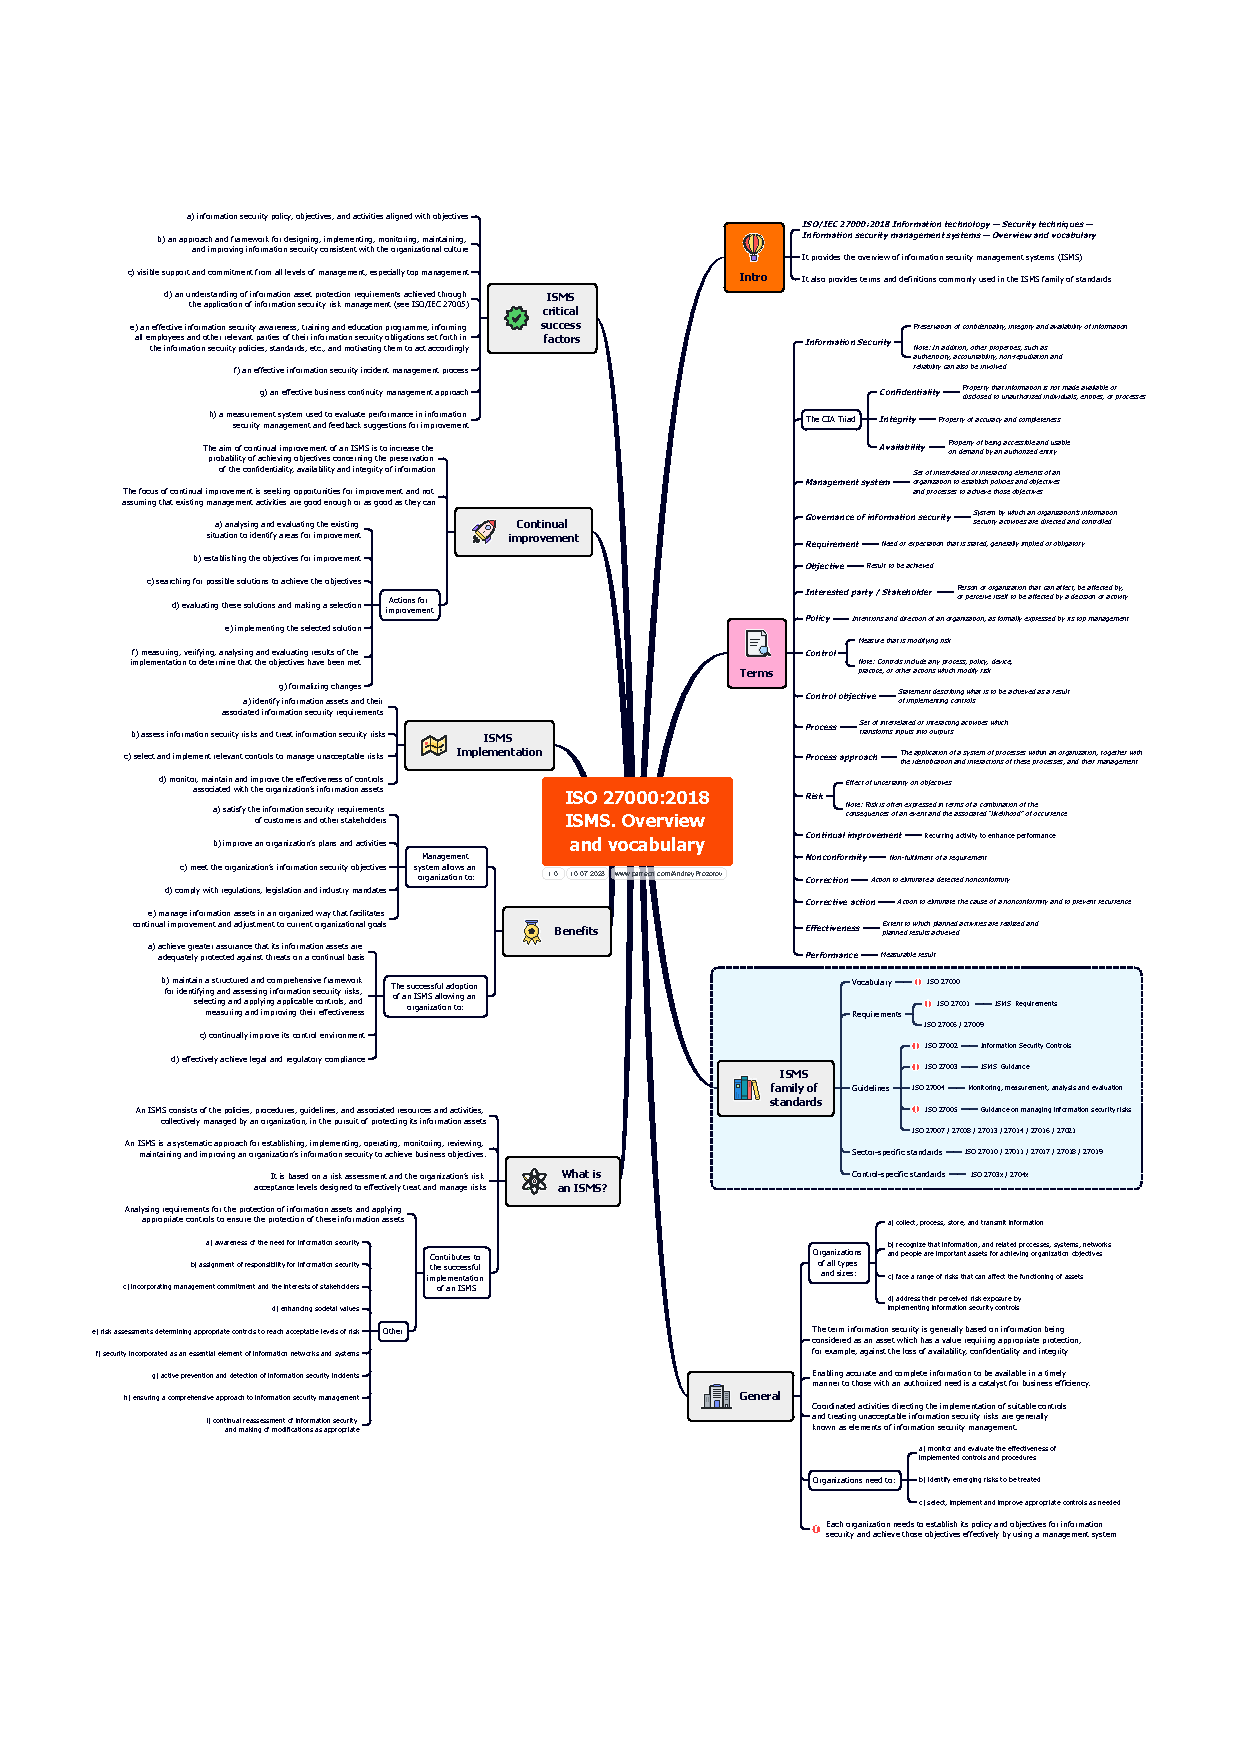
\includepdf[pages={1-6},pagecommand={\thispagestyle{fancy}}, fitpaper=true]{./appendices/iso-27k-mindmaps}
     %\end{appendices}
\end{document}





                                                          

               

  